\chapter{Medições}

O InVesalius permite realizar medições lineares e angulares em 2D (planos axial,
coronal e sagital) e em 3D (superfícies). Também é possível fazer medições
volumétricas em superfícies.

\section{Medição linear}

Para realizar medições lineares, é necessário ativar o recurso clicando no atalho
correspondente localizado na barra de ferramentas (figura \ref{fig:measure_line_original}).

\begin{figure}[!htb]
\centering

\includegraphics[scale=0.2]{measure_line_original}
\caption{Atalho para ativar medição linear}
\label{fig:measure_line_original}
\end{figure}

Uma medição linear é definida entre dois pontos. Com o recurso ativado, clique
\textbf{uma} vez sobre a imagem para estabelecer o ponto inicial. Em seguida,
posicione o ponteiro do mouse no ponto final e clique \textbf{uma} vez novamente.
A medição é executada e o resultado é exibido automaticamente sobre a imagem ou
superfície.

A figura \ref{fig:axial_linear} mostra uma medida linear em 2D na orientação axial,
e a figura \ref{fig:3d_linear} mostra outra medida linear em 3D (superfície).

Uma vez feita a medida linear em 2D, é possível edita-la, para isso é necessário posicionar o mouse sobre uma das extremidades, manter o \textbf{botão direito do mouse} pressionado e arrastar para a posição desejada.

\begin{figure}[!htb]
\centering
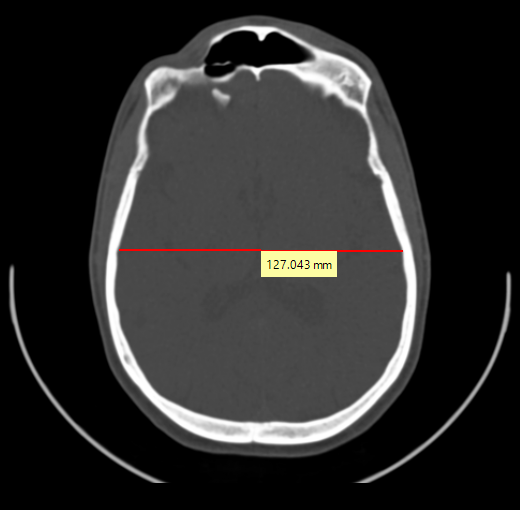
\includegraphics[scale=0.4]{axial_linear.png}
\caption{Medida linear sobre imagem plana}
\label{fig:axial_linear}
\end{figure}

\begin{figure}[!htb]
\centering
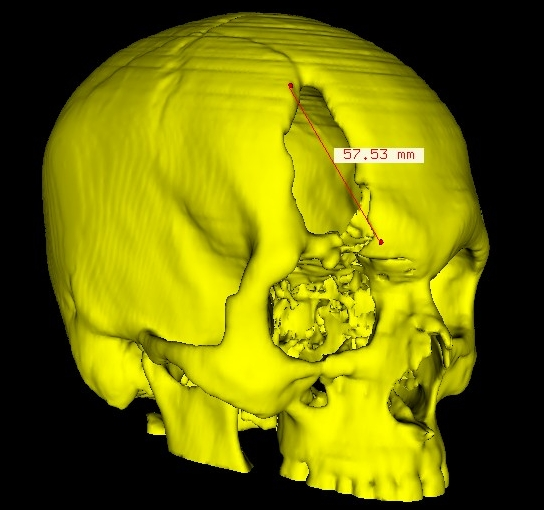
\includegraphics[scale=0.3]{3d_linear.jpg}
\caption{Medida linear sobre superfície}
\label{fig:3d_linear}
\end{figure}

\textbf{Nota: A medida linear é dada em milímetros (mm).}

\section{Medição angular}

Uma medição angular em 2D ou sobre uma superfície (3D) pode ser realizada clicando-se
no atalho ilustrado na figura \ref{fig:atalho_angular}.

\begin{figure}[!htb]
\centering

\includegraphics[scale=0.2]{measure_angle_original}
\caption{Atalho para medição angular}
\label{fig:atalho_angular}
\end{figure}

Para efetuar a medição angular, é necessário fornecer os três pontos que descreverão o
ângulo a ser medido, A\^{B}C. Posicione o ponteiro do mouse e clique \textbf{uma} vez
com o botão esquerdo para determinar o primeiro ponto, A. Para inserir o segundo ponto,
B (o vértice do ângulo ou o "centro do transferidor"), posicione o ponteiro do mouse e
clique \textbf{uma} vez novamente. Repita as mesmas ações para determinar o terceiro
ponto, C. A medição é executada e, automaticamente, a medida resultante é exibida sobre
a imagem ou superfície.

A figura \ref{fig:axial_angular} ilustra uma medida angular em uma imagem plana, e a
figura \ref{fig:axial_superficie} ilustra uma medida angular sobre uma superfície.

A exemplo da medida linear em 2D, também é possível editar a medida angular 2D, para isso é necessário posicionar o mouse sobre uma das extremidades, manter o \textbf{botão direito do mouse} pressionado e arrastar para a posição desejada.

\begin{figure}[!htb]
\centering
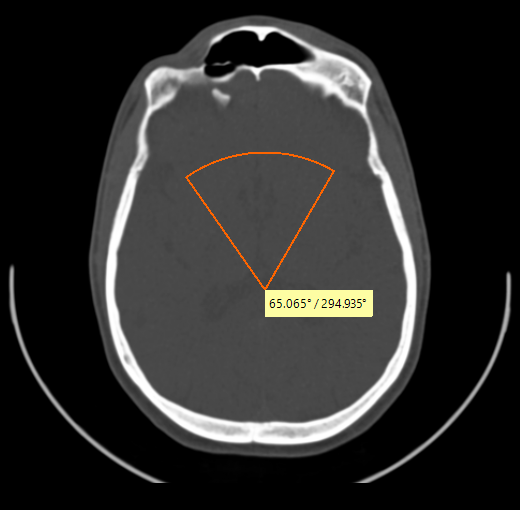
\includegraphics[scale=0.38]{axial_angular.png}
\caption{Medida angular sobre imagem plana}
\label{fig:axial_angular}
\end{figure}

\begin{figure}[!htb]
\centering
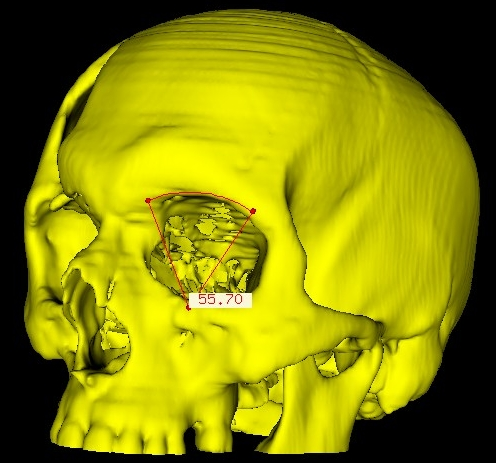
\includegraphics[scale=0.33]{angular_superficie.jpg}
\caption{Medida angular sobre superfície}
\label{fig:axial_superficie}
\end{figure}

\textbf{Nota: A medida angular é dada em graus ($^{\circ}$)}


\section{Medição volumétrica}

As medições de volume e área são feitas automaticamente ao se criar uma nova superfície.
Elas são exibidas na aba \textbf{Superfícies 3D}, no painel de gerenciamento de \textbf{Dados}, localizado no canto
inferior esquerdo da tela, como ilustra a figura \ref{fig:volumetric_mensure}.

\begin{figure}[!htb]
\centering
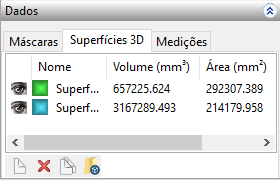
\includegraphics[scale=0.7]{painel_volumetric_measures_pt.png}
\caption{Medidas volumétricas}
\label{fig:volumetric_mensure}
\end{figure}

\textbf{Nota: A medida de volume é dada em milímetro cúbico ($mm^3$), já a de área em milímetro quadrado ($mm^2$)}
